\documentclass{article}
\usepackage{graphicx}
\title{ECE 1895 - ASSIGNMENT 6 REPORT}
\author{Yinhao Qian}
\begin{document}
	\maketitle
	\section{Explanation}
	\subsection{What does it do?}
	Just as what the project name on the PCB suggests, it's a dual-frequency buzzer. Once the power source and a stable ground are connected, the buzzer will go off in one of the two frequencies based on the position of the switch. This simple design can be used in many fields in the real-world, such as subway platform door alarm. 
	\subsection{How does it work?}
	The 555 timer will output a frequencies of square waves, and the frequencies have 2 options, which are all calculated so that the output frequencies are desired for the buzzer. Two capacitors are implemented as low pass filters to make sure the signals output is stable. The switch will control which resistor the current will flow through, which is the determining factor of the frequencies of square wave the 555-timer will produce, and finally, the buzzer will produce the sound according to the frequencies given. 
	\section{Best Practice}
	I have made changes to the PCB design according to \textbf{LECTURE M3 SLIDES P13}, so that the original rectangular design have been changed to a square design to minimize the production cost. At the same time, I have also made the layout of components way more compact than ever. (Layout design are in the PCB Section). At the same time, since it's not a industry-based project, I have eliminated some non-critical capacitors so that less components will be implemented.\newline
	As also mentioned during lecture, my previous designed uses surface mount components, which can be very difficult to install, and that's why in this design have I replaced all of them with through-hole design.
	\section{Screenshots}
	\subsection{Schematic}
	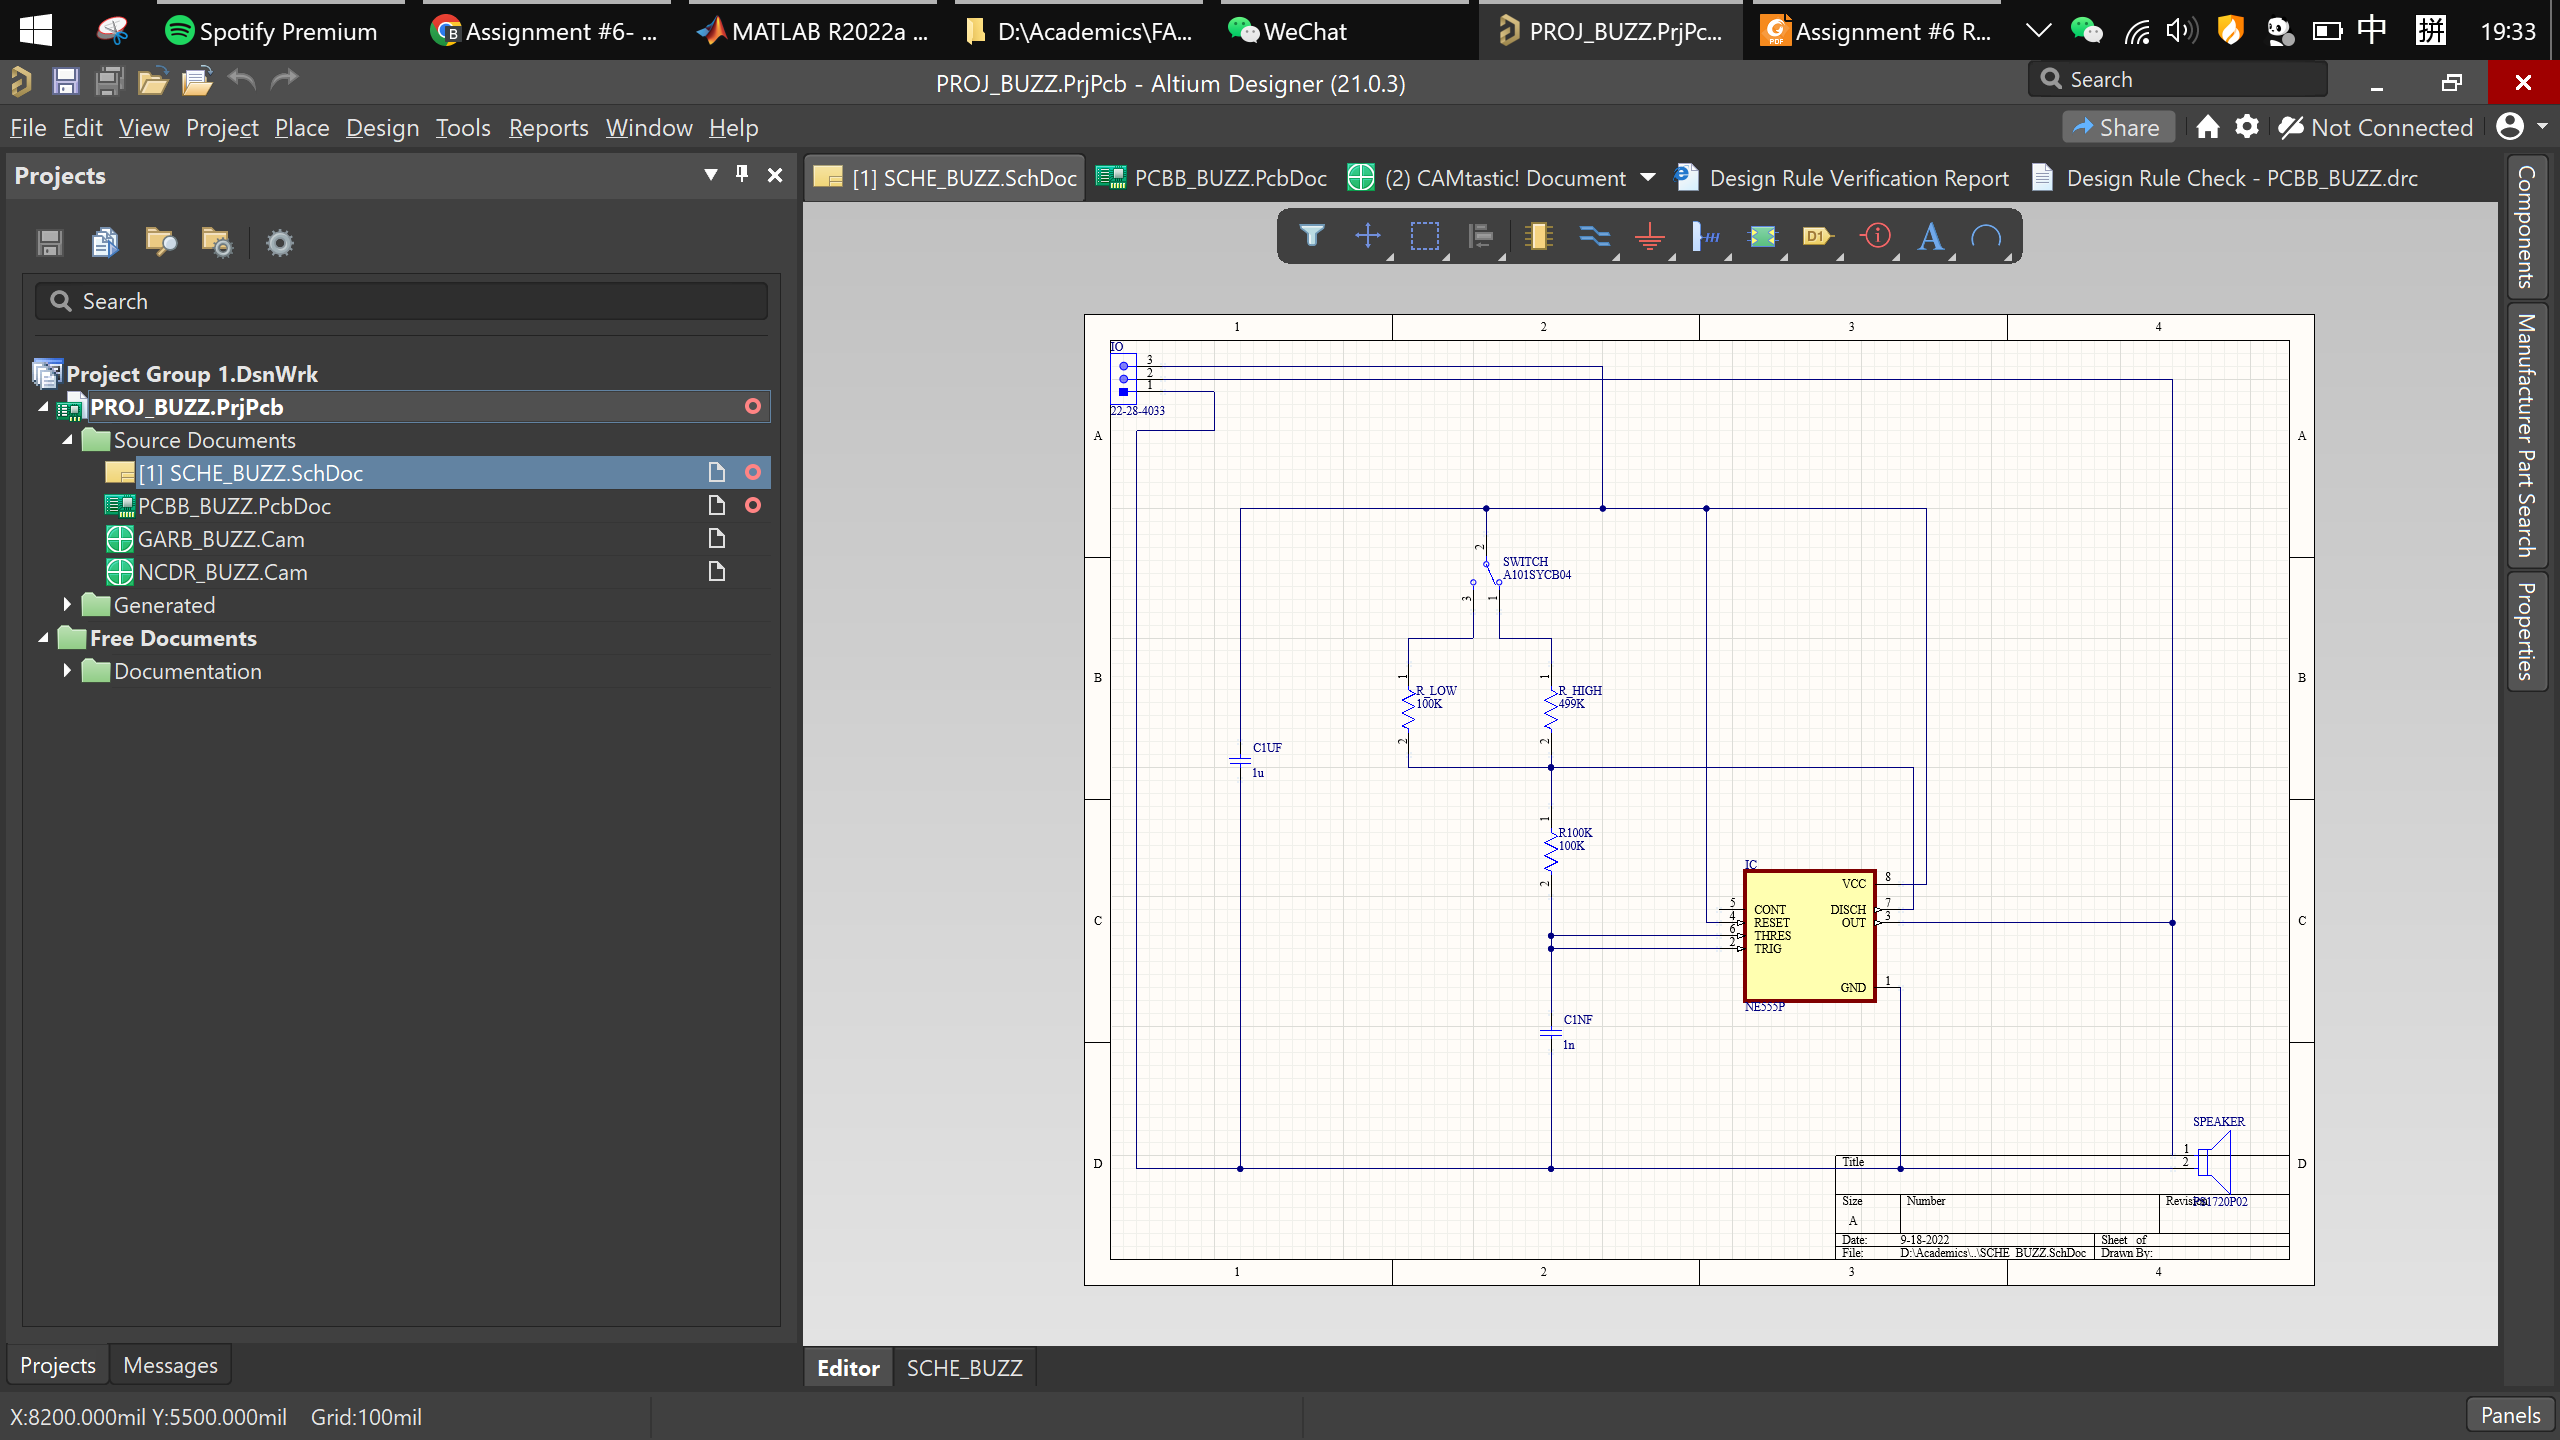
\includegraphics[width=\columnwidth]{SCHE}
	\subsection{PCB}
	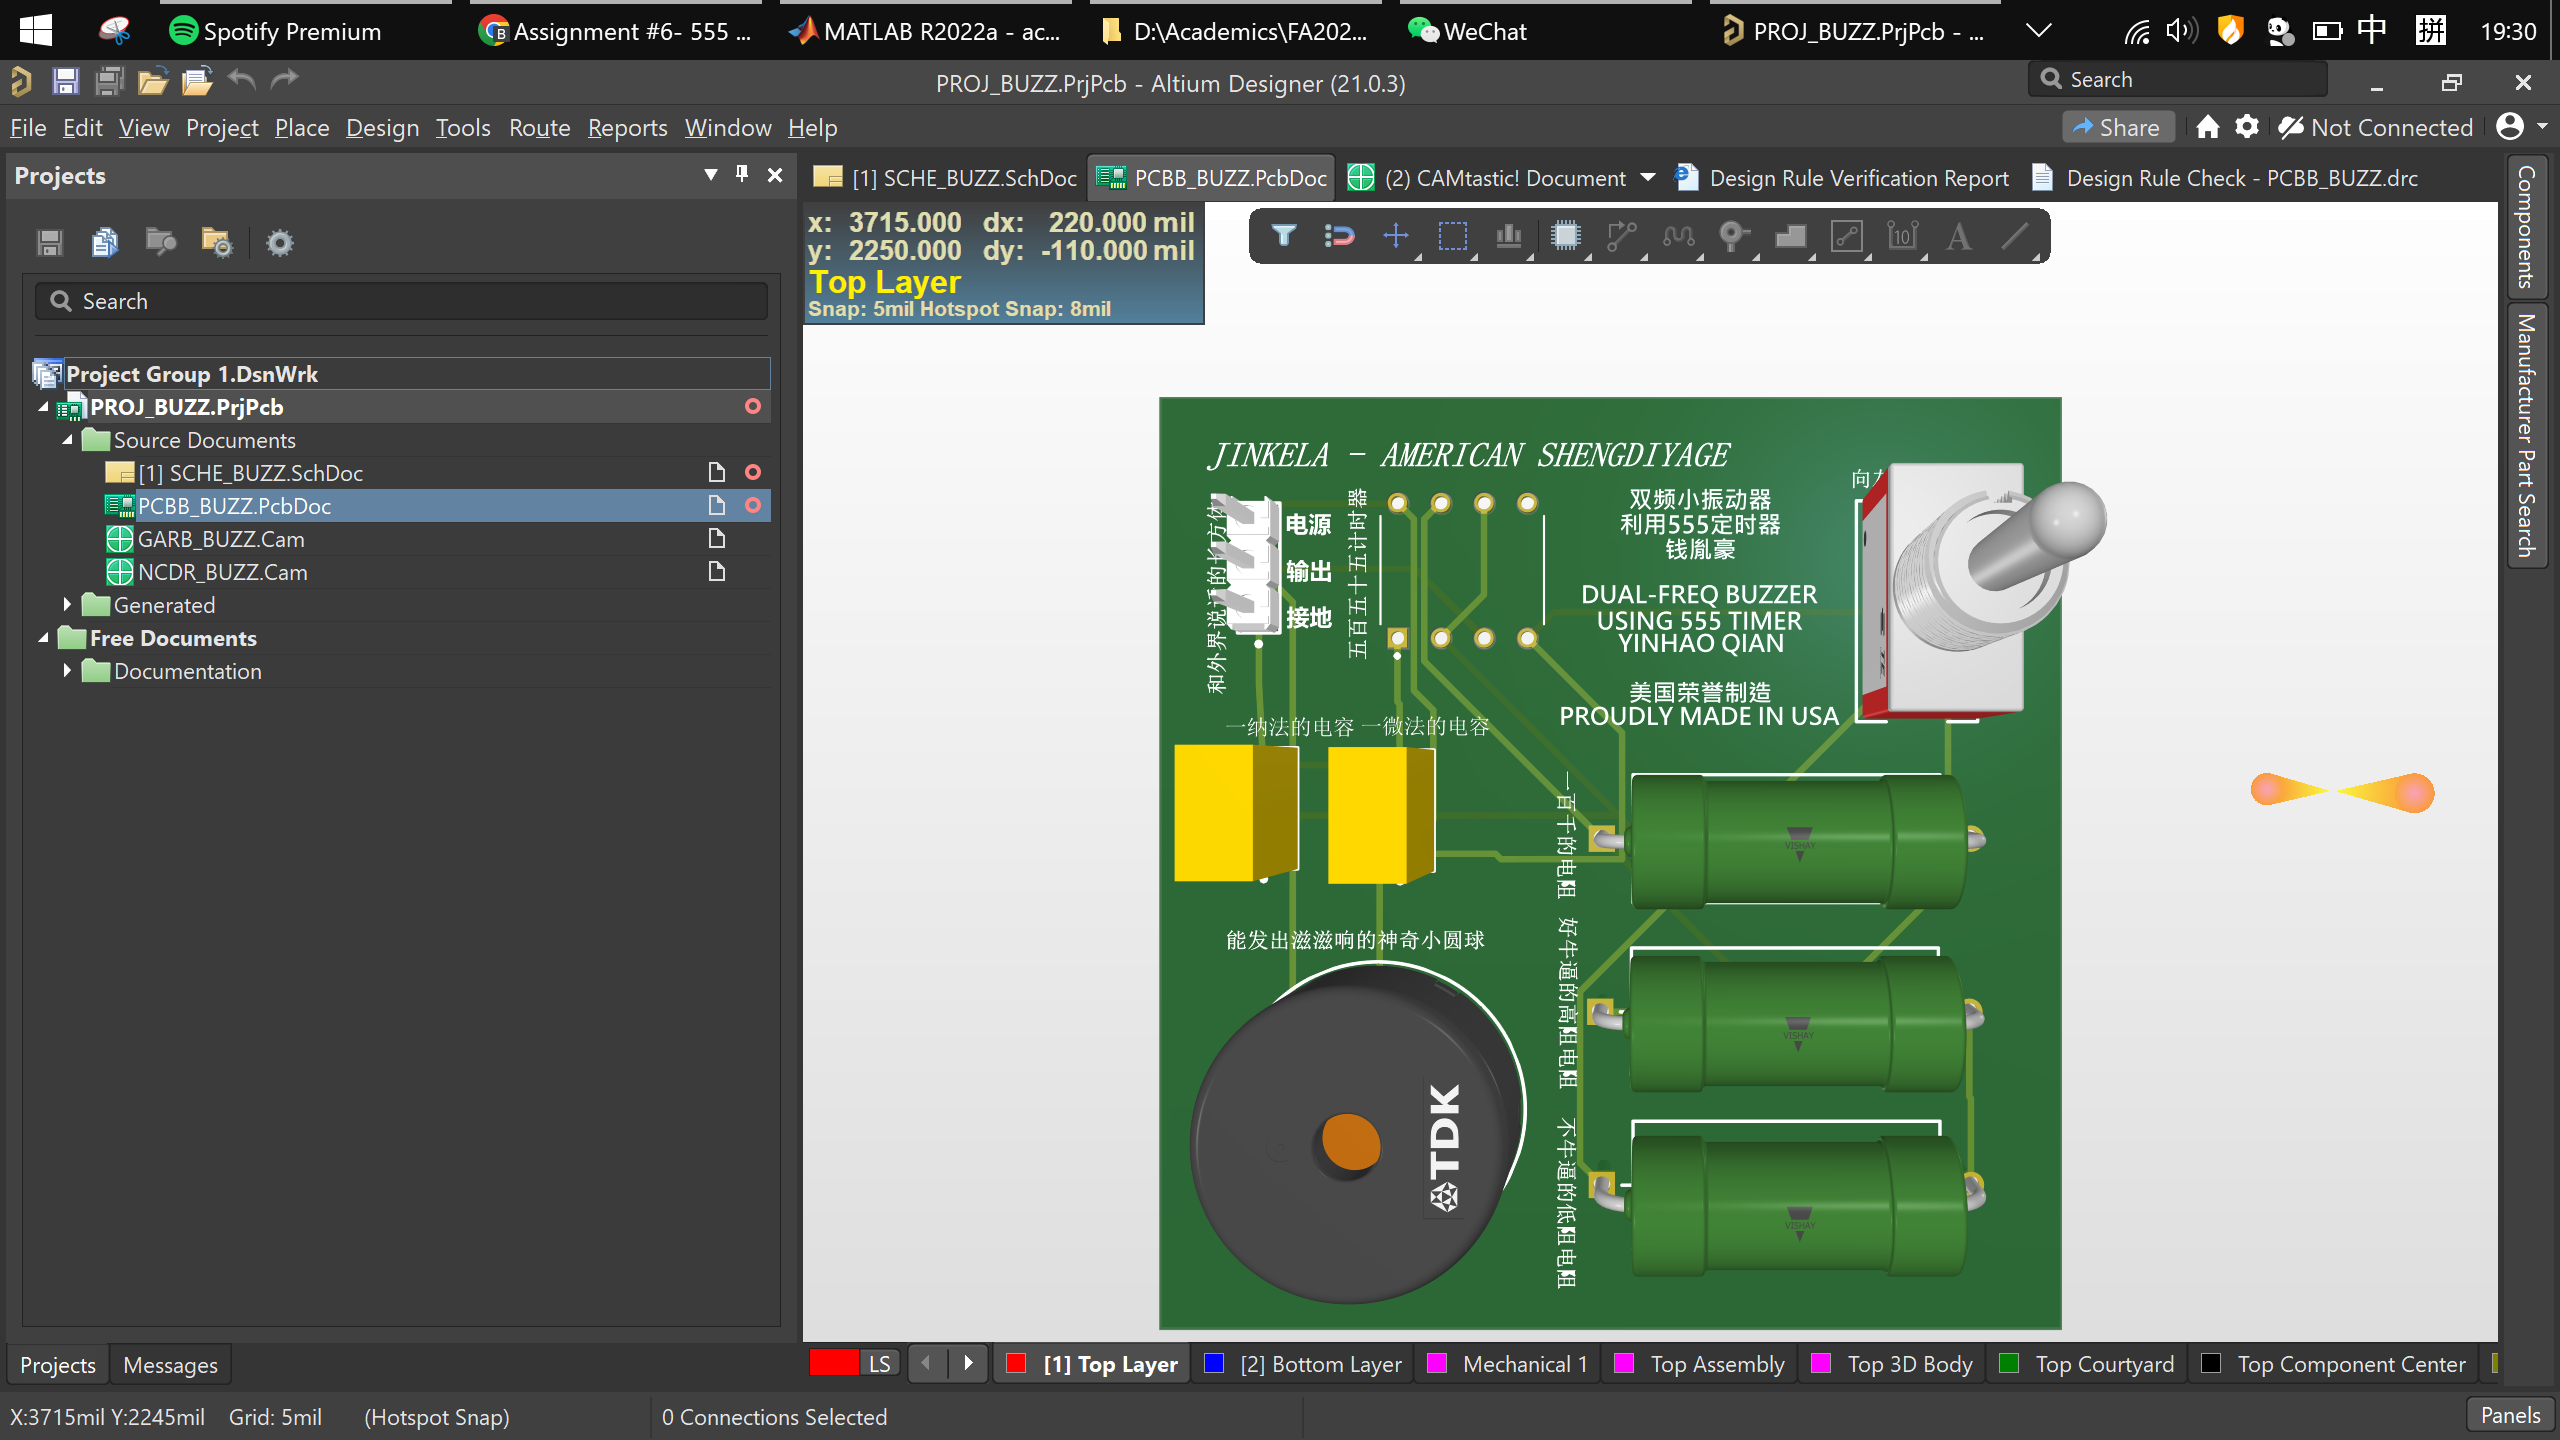
\includegraphics[width=\columnwidth]{PCBB}
	\subsection{Oskpark Verification}
	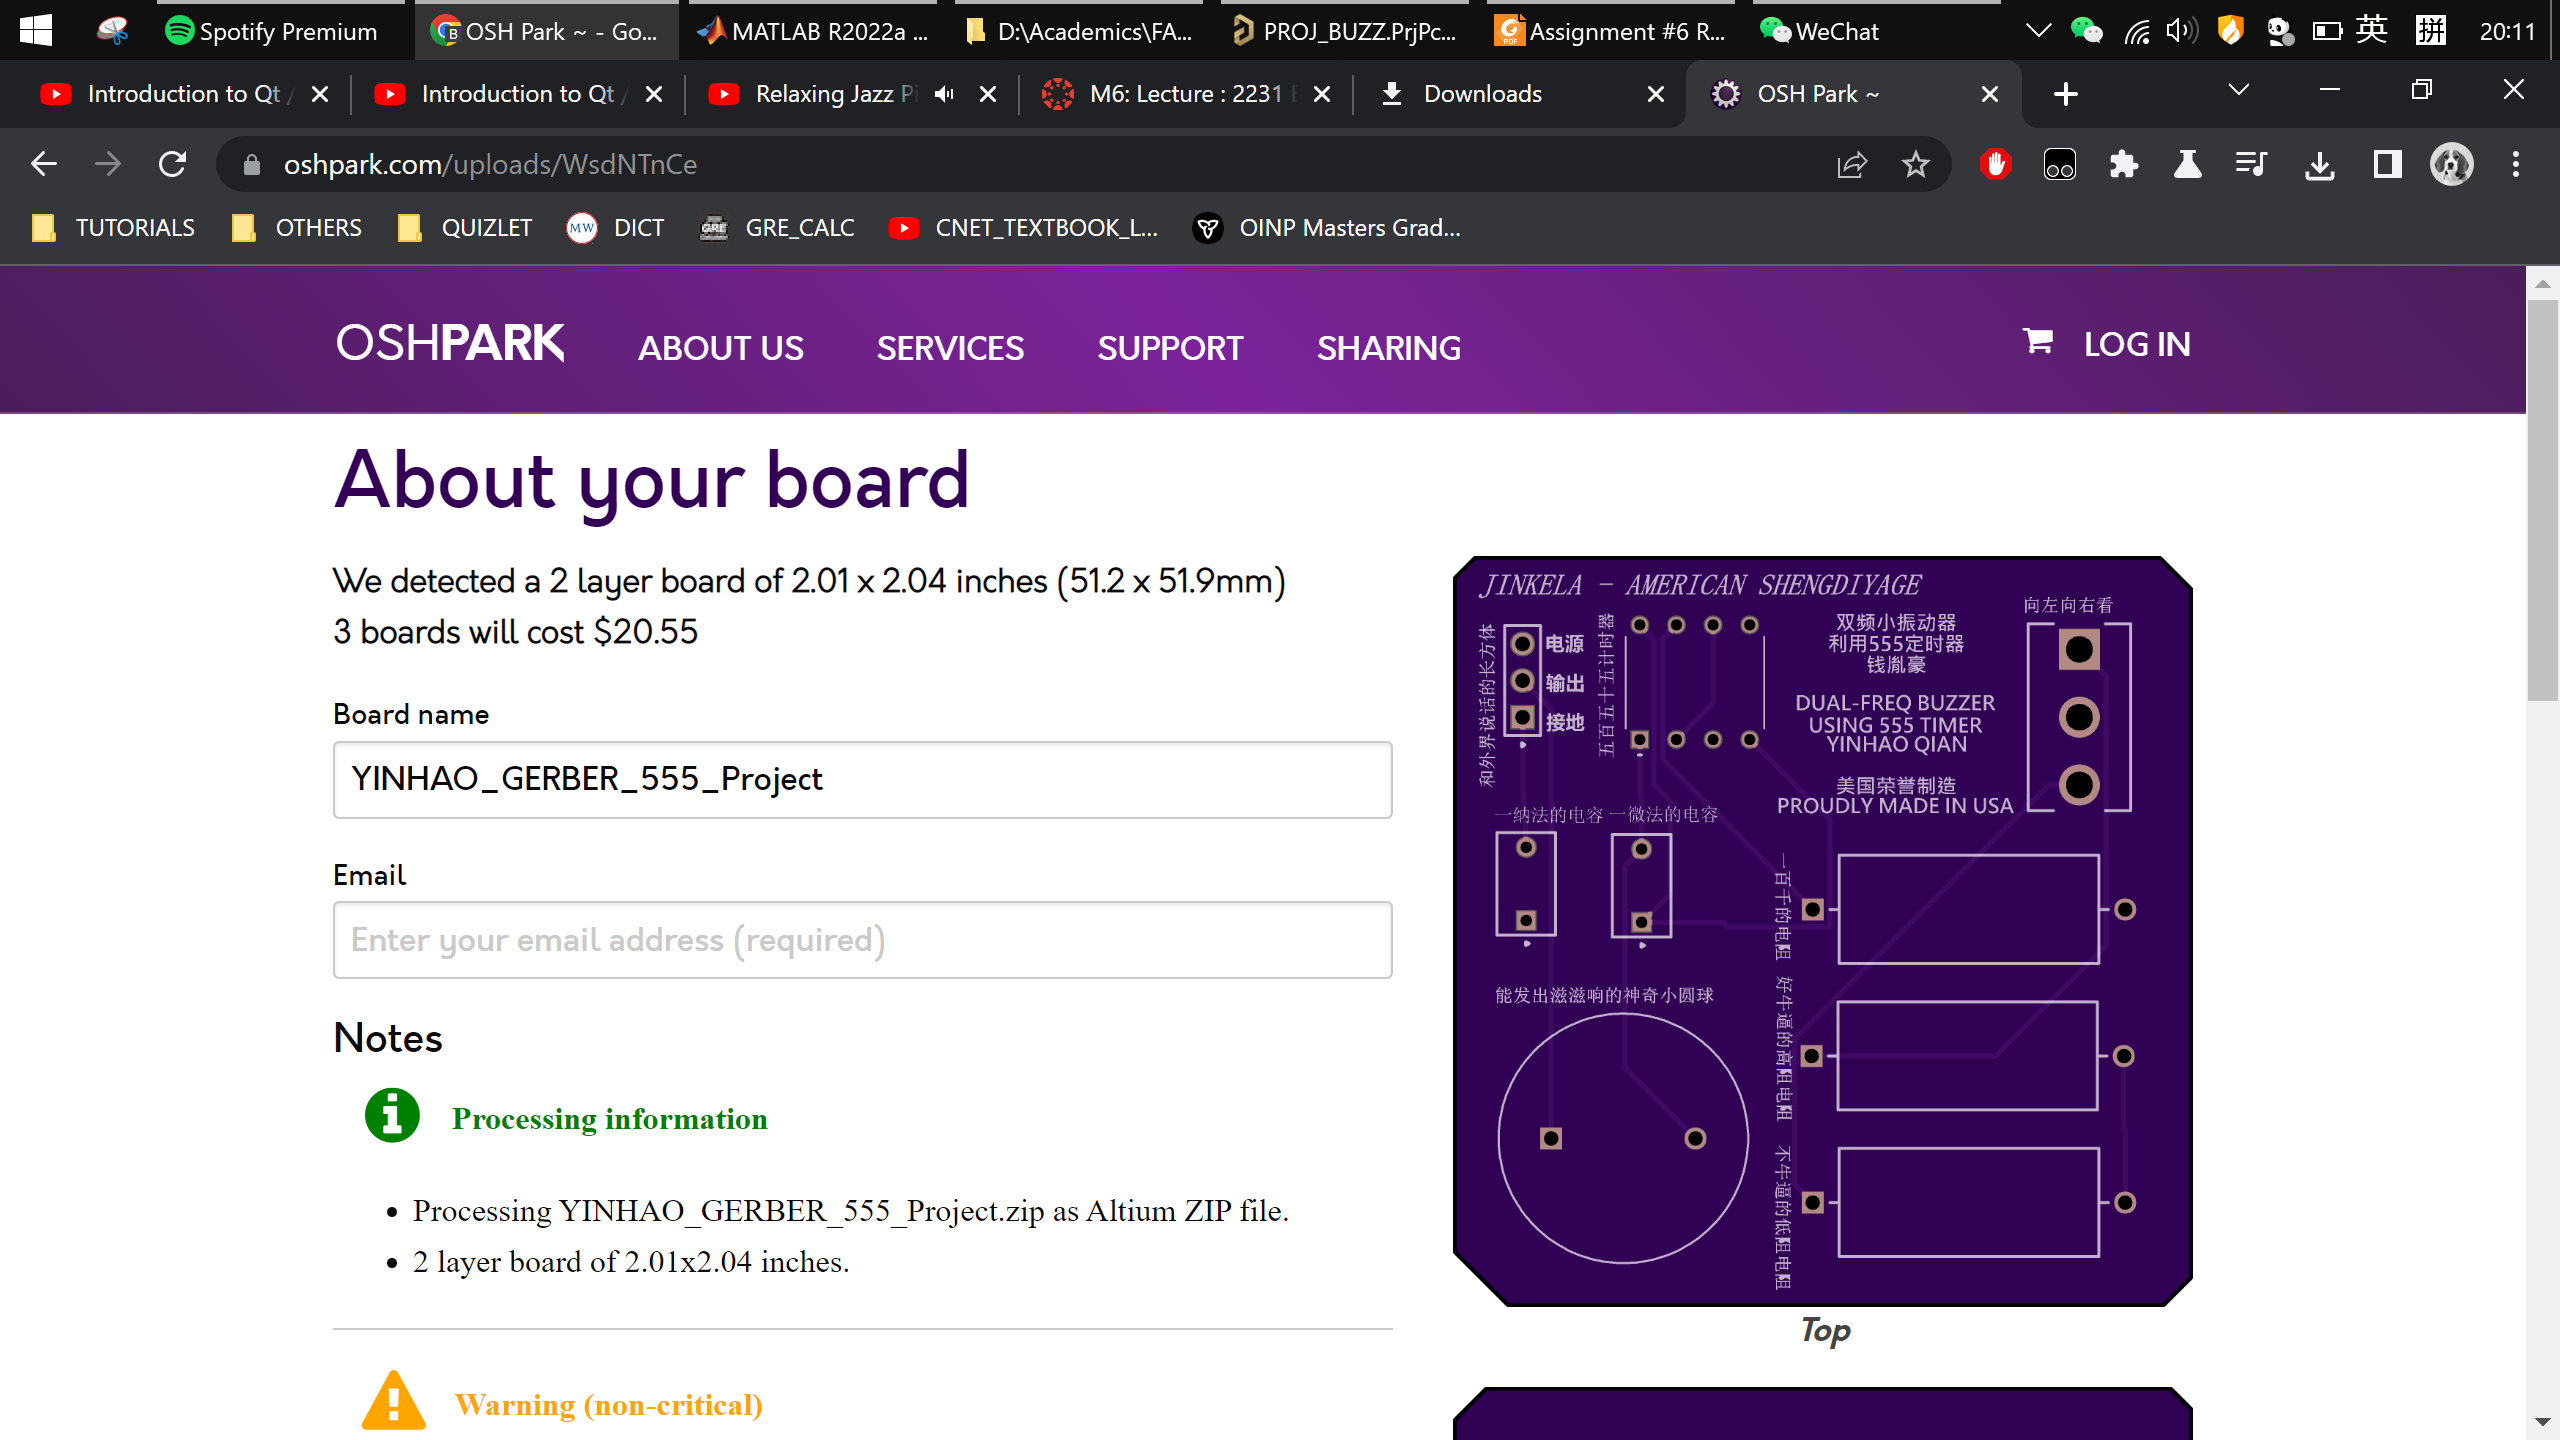
\includegraphics[width=\columnwidth]{OSHP}
\end{document}